\documentclass{standalone}

\usepackage[dvipsnames]{xcolor}
\usepackage{contour}
\contournumber{2048}
\contourlength{0.05ex}

\usepackage{tikz}
\usetikzlibrary{intersections}

\colorlet{wcolor}{CornflowerBlue}
\pagecolor{white}
\Huge
\newlength{\inl}
\setlength{\inl}{0.80ex}%{0.66ex}

\usepackage{fontspec}
\setmainfont{Bilbo Swash Caps}%{HoltwoodOneSC}%{Roboto Slab-Black}
\begin{document}

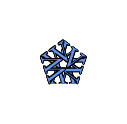
\begin{tikzpicture}[rotate=180]
	\node[rotate=180] at (90:\inl) {\contour{black}{\textcolor{wcolor}{W}}};
	\node[rotate=252] at (162:\inl) {\contour{black}{\textcolor{wcolor}{W}}};
	\node[rotate=324] at (234:\inl) {\contour{black}{\textcolor{wcolor}{W}}};
	\node[rotate=36] at (306:\inl) {\contour{black}{\textcolor{wcolor}{W}}};
	\node[rotate=108] at (18:\inl) {\contour{black}{\textcolor{wcolor}{W}}};
	
%	\draw[line width=0.275ex] (120:2.25ex) -- (60:2.25ex) -- (0:2.25ex) -- (300:2.25ex) -- (240:2.25ex) -- (180:2.25ex) -- cycle;
%	\draw[line width=0.2ex] (0,0) circle (2.1ex);
\end{tikzpicture}

\end{document}